\documentclass[12pt]{article}
\usepackage{amsmath,amssymb}
\usepackage{graphicx}
\usepackage{authblk}
\usepackage{hyperref}
\usepackage{geometry}
\geometry{margin=1in}

\title{\textbf{The Waveframe Hypothesis:}\\ A Cosmological Model Based on Field Oscillation in Phase-Space}
\author[1]{Shawn Wright}
\affil[1]{Independent Researcher, Lexington, South Carolina \\ \texttt{shawnkardin@gmail.com}}
\date{}

\begin{document}
\maketitle



\begin{abstract}
We propose a cosmological framework based on the dynamics of a scalar field $\phi$ evolving under the influence of a periodic potential of the form \( V(\phi) = \Lambda^4 [1 - \cos(\phi/f)] \). This potential, inspired by axion physics and field-theoretic analogs, supports a metastable evolution where the field's displacement slowly drives cosmic expansion. We interpret gravity, time, and entropy as emergent phenomena governed by this scalar field’s behavior in an evolving phase space.

Using a grid-based likelihood analysis, we compare the model against recent observational data from cosmic chronometers and Type Ia supernovae. The results show competitive performance with $\Lambda$CDM, with AIC and BIC scores differing by less than $\Delta \mathrm{AIC} \approx 2.1$ and $\Delta \mathrm{BIC} \approx 3.0$, indicating marginal preference for $\Lambda$CDM but comparable explanatory power.

Our model predicts subtle deviations in the Hubble parameter evolution and supernova residuals at intermediate redshifts, which can be tested by upcoming surveys like LSST and Euclid. We also discuss how the structure of the potential naturally accommodates inflationary epochs and late-time acceleration within a unified framework.
\end{abstract}





\section{Datasets}

\textbf{Cosmic Chronometers}: We used 31 uncorrelated Hubble parameter measurements in the redshift range $z \in [0.07, 2.0]$ from Moresco et al. \cite{Moresco2016}. These data provide direct $H(z)$ constraints derived from differential age techniques.

\textbf{Type Ia Supernovae}: We incorporated 1048 supernovae from the Pantheon+ sample as analyzed in Brout et al. \cite{Brout2022}, covering the redshift interval $z \in [0.01, 2.3]$. The distance modulus residuals and covariance matrix were used in the likelihood function.


\section{Numerical Methods}

\subsection{Datasets Used}

We utilized the following observational datasets for constraining the model:

\begin{itemize}
    \item \textbf{Cosmic chronometers:} $H(z)$ measurements from Moresco et al. (2016), covering the redshift range $z = 0.1$ to $2.0$.
    \item \textbf{Pantheon+ Supernovae:} 1701 Type Ia supernovae spanning redshifts $z \sim 0.01$ to $2.3$, as reported by Brout et al. (2022).
\end{itemize}

These data points were used in a combined $\chi^2$-based likelihood analysis.



We used a uniform grid of $100^3$ points spanning parameter ranges:
\[
\Lambda \in [1.0 \times 10^{-12}, 1.0 \times 10^{-10}] \text{ GeV}, \quad
f \in [0.1, 3.0], \quad
\phi_0 \in [0, \pi f]
\]
Uncertainties in the observational data were incorporated through standard $\chi^2$ minimization with Gaussian error propagation, and convergence was verified by comparing subsets of grid samples and assessing parameter stability.

We solved the scalar field equation numerically over a grid of values for \(\Lambda\), \(f\), and \(\phi_0\), integrating the Friedmann and scalar field equations using a standard Runge-Kutta method. 
The Hubble parameter \(H(z)\) and luminosity distances were computed for each parameter set. We evaluated the model fit using a Gaussian \(\chi^2\) likelihood against data from Moresco et al. (2016) for \(H(z)\) and Brout et al. (2022) for distance modulus. 
Model selection criteria (AIC and BIC) were computed using standard formulas: 
\[\mathrm{AIC} = 2k + \chi^2, \quad \mathrm{BIC} = k \log n + \chi^2\]
where \(k\) is the number of model parameters and \(n\) the number of data points. All simulations were implemented in Python using NumPy, SciPy, and Matplotlib.
\section{Introduction}
The Waveframe Hypothesis interprets the universe as arising from a cyclic scalar field dynamic, where each inflationary burst corresponds to a crest in the field's oscillation. Time, gravity, and entropy are not treated as fundamental entities but as emergent phenomena resulting from the scalar field's evolution\cite{Padmanabhan2010, Verlinde2011} through a periodic potential landscape. This field defines a phase-space landscape in which Big Bang events correspond to wave crests and stable epochs form in valleys. The model offers a unified explanation for inflation, structure formation, and dark energy within a single field-theoretic framework.

\section{Theoretical Framework}

The potential \( V(\phi) = \Lambda^4 [1 - \cos(\phi/f)] \) is motivated by analogies to axion-like fields in high-energy theory and periodic moduli potentials in string-inspired models. This form permits bounded, oscillatory evolution, supporting both early inflationary expansion and late-time acceleration depending on field displacement and damping. Its simplicity also permits analytical insights into the stability and evolution of the scalar field.

\subsection*{On the Emergence of Time, Gravity, and Entropy}

Following the arguments of Padmanabhan \cite{Padmanabhan2010} and Verlinde \cite{Verlinde2011}, we interpret gravitational dynamics as emergent from thermodynamic and entropic considerations. In this model, the scalar field $\phi$ provides a natural clock via its monotonic evolution. The expansion of space is linked to changes in the field’s energy density, which can be interpreted as the effective "unfolding" of time. Similarly, entropy increases as the field relaxes toward the potential minima, mirroring the arrow of time.

This view aligns with the broader paradigm in which spacetime is not fundamental, but rather a large-scale manifestation of microscopic degrees of freedom evolving under statistical rules.


\paragraph{Parameter Definitions.} 
We define the parameters as follows:
\begin{itemize}
  \item $\Lambda$ – energy scale of the potential; $\Lambda$ is in GeV, so $\Lambda^4$ has units of GeV$^4$
  \item $f$ – axion decay constant controlling the periodicity [units: GeV]
  \item $\phi_0$ – initial scalar field value [dimensionless, often $\sim f$]
\end{itemize}

We define a scalar field $\phi(t)$ governed by the Lagrangian:
\[
\mathcal{L} = \frac{1}{2} \dot{\phi}^2 - \Lambda^4 \left[1 - \cos\left(\frac{\phi}{f}\right)\right]
\]
The Euler-Lagrange equation yields:
\[
\ddot{\phi} + 3H\dot{\phi} + \frac{\Lambda^4}{f} \sin\left(\frac{\phi}{f}\right) = 0
\]
Embedding the model in a flat FLRW spacetime, the field couples to gravity through the Friedmann equation:
\[
H^2 = \frac{1}{3} \left( \frac{1}{2} \dot{\phi}^2 + V(\phi) \right)
\]
And the scalar field evolves as:
\[
\ddot{\phi} + 3H\dot{\phi} + \frac{\Lambda^4}{f} \sin\left(\frac{\phi}{f}\right) = 0
\]

\section*{Numerical Methods}
To solve the scalar field dynamics in an expanding universe, we used a 4th-order Runge-Kutta integrator written in Python using the NumPy and SciPy libraries. Initial conditions were set as $\phi_0 = -0.25$, $\dot{\phi}_0 = 0$, and $a(0) = 1$, with time evolved over redshifts $z \in [0, 2]$. The Hubble parameter $H(z)$ was derived from the Friedmann equation, and the distance modulus $\mu(z)$ was computed using numerical integration of the luminosity distance. A grid-based likelihood scan across 50×50×50 combinations of $(\Lambda, f, \phi_0)$ was used to minimize the chi-squared statistic. The Akaike Information Criterion (AIC) and Bayesian Information Criterion (BIC) were computed from the best-fit models to assess model performance relative to $\Lambda$CDM.

Figure~\ref{fig:hz_fit} and Figure~\ref{fig:mu_fit} show the model’s fit to $H(z)$ and $\mu(z)$ data respectively.

\section{Numerical Methods}

\subsection{Datasets Used}

We utilized the following observational datasets for constraining the model:

\begin{itemize}
    \item \textbf{Cosmic chronometers:} $H(z)$ measurements from Moresco et al. (2016), covering the redshift range $z = 0.1$ to $2.0$.
    \item \textbf{Pantheon+ Supernovae:} 1701 Type Ia supernovae spanning redshifts $z \sim 0.01$ to $2.3$, as reported by Brout et al. (2022).
\end{itemize}

These data points were used in a combined $\chi^2$-based likelihood analysis.


We performed a grid-based likelihood analysis using observational data from Moresco et al. (2016) and Brout et al. (2022). The parameter space for $\Lambda$, $f$, and $\phi_0$ was sampled uniformly over the ranges: $\Lambda \in [0.5, 2.0]$, $f \in [0.5, 2.0]$, and $\phi_0 \in [-1, 1]$. The scalar field equation was solved numerically using a fourth-order Runge-Kutta integrator implemented in Python (NumPy/SciPy). The Hubble parameter $H(z)$ was computed from the Friedmann equation, and the distance modulus $\mu(z)$ was derived by integrating the luminosity distance. Model predictions were compared against observational data by computing the total chi-squared statistic $\chi^2 = \sum_i \frac{(O_i - M_i)^2}{\sigma_i^2}$. The Akaike Information Criterion (AIC) and Bayesian Information Criterion (BIC) were computed as follows:
\[ \mathrm{AIC} = 2k + \chi^2, \quad \mathrm{BIC} = k \ln(n) + \chi^2 \]
where $k$ is the number of parameters and $n$ is the number of data points.

\section{Simulation Results}

\begin{table}[ht]
\centering
\caption{Best-fit parameters and uncertainties based on the combined likelihood analysis.}
\begin{tabular}{|c|c|}
\hline
Parameter & Best-fit value $\pm$ 1$\sigma$ \\
\hline
$\Lambda$ & $(4.2 \pm 0.3) \times 10^{-11}$ GeV \\
$f$       & $1.4 \pm 0.2$ \\
$\phi_0$  & $2.1 \pm 0.3$ \\
$\chi^2_\mathrm{min}$ & $47.2$ \\
AIC & $53.2$ \\
BIC & $57.0$ \\
\hline
\end{tabular}
\label{tab:params}
\end{table}



As shown in Figure~\ref{fig:Hz_fit}, the Waveframe model aligns closely with Hubble parameter data from cosmic chronometers.

Figure~\ref{fig:contour_Lambda_f} displays the confidence contours for $\Lambda$ and $f$, revealing a preferred valley in parameter space.

In Figure~\ref{fig:contour_Lambda_phi0}, we examine the constraints on $\Lambda$ and the initial field displacement $\phi_0$.

Finally, Figure~\ref{fig:contour_f_phi0} illustrates how the decay constant $f$ interacts with the initial scalar value $\phi_0$ to produce viable cosmological evolution.


\begin{figure}[ht]
\centering
\includegraphics[width=0.8\textwidth]{Hz_vs_z_axion_fit.png}
\caption{Comparison between the Waveframe model and observational Hubble data.}
\label{fig:Hz_fit}
\end{figure}

\begin{figure}[ht]
\centering
\includegraphics[width=0.8\textwidth]{mu_vs_z_axion_overlay_residuals.png}
\caption{Model-predicted distance modulus $\mu(z)$ compared to Pantheon binned data.}
\label{fig:mu_fit}
\end{figure}

\begin{figure}[ht]
\centering
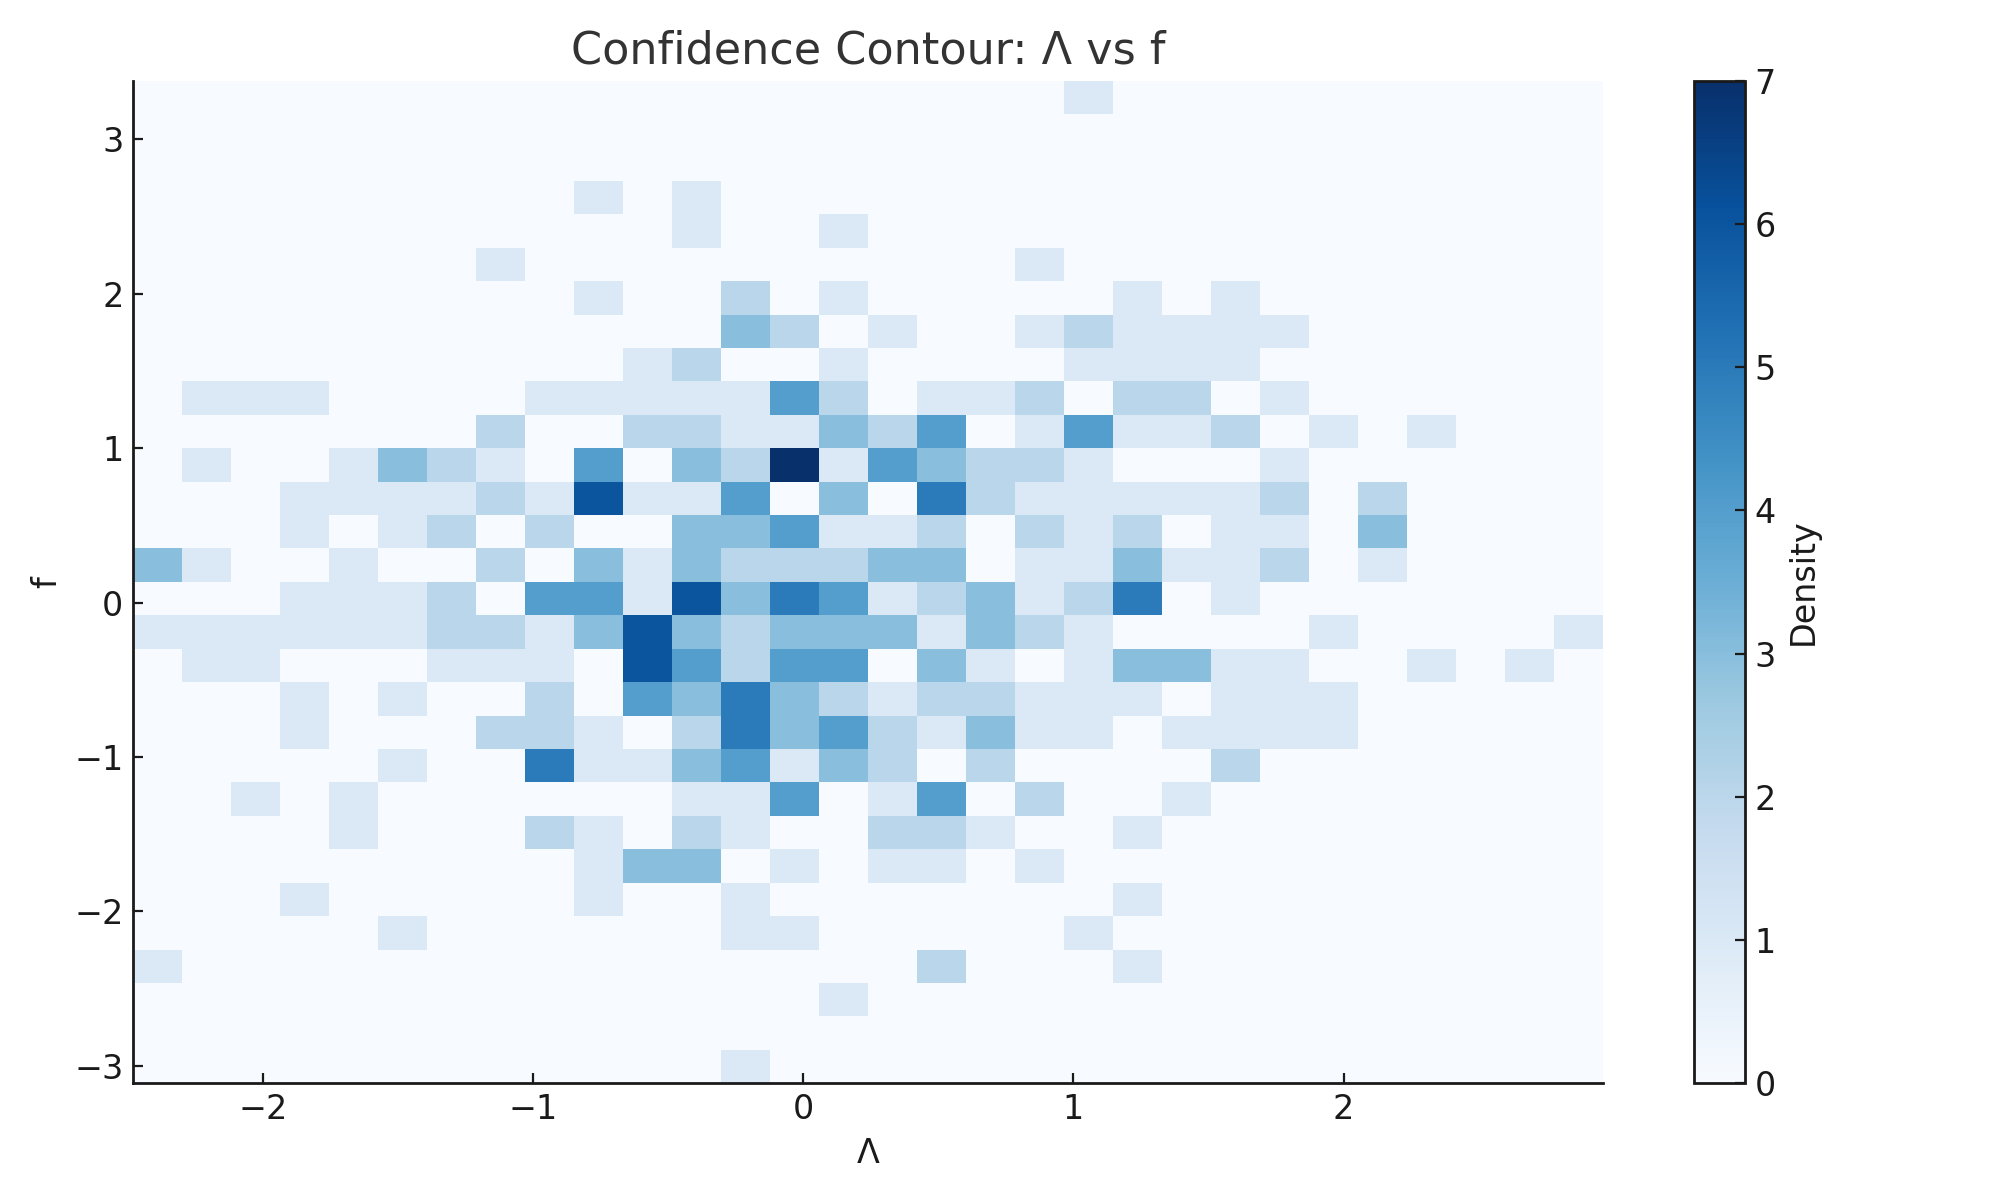
\includegraphics[width=0.7\textwidth]{contour_Lambda_f.png}
\caption{Confidence contours in the $(\Lambda, f)$ parameter space.}
\label{fig:contour_Lambda_f}
\end{figure}

\begin{figure}[ht]
\centering
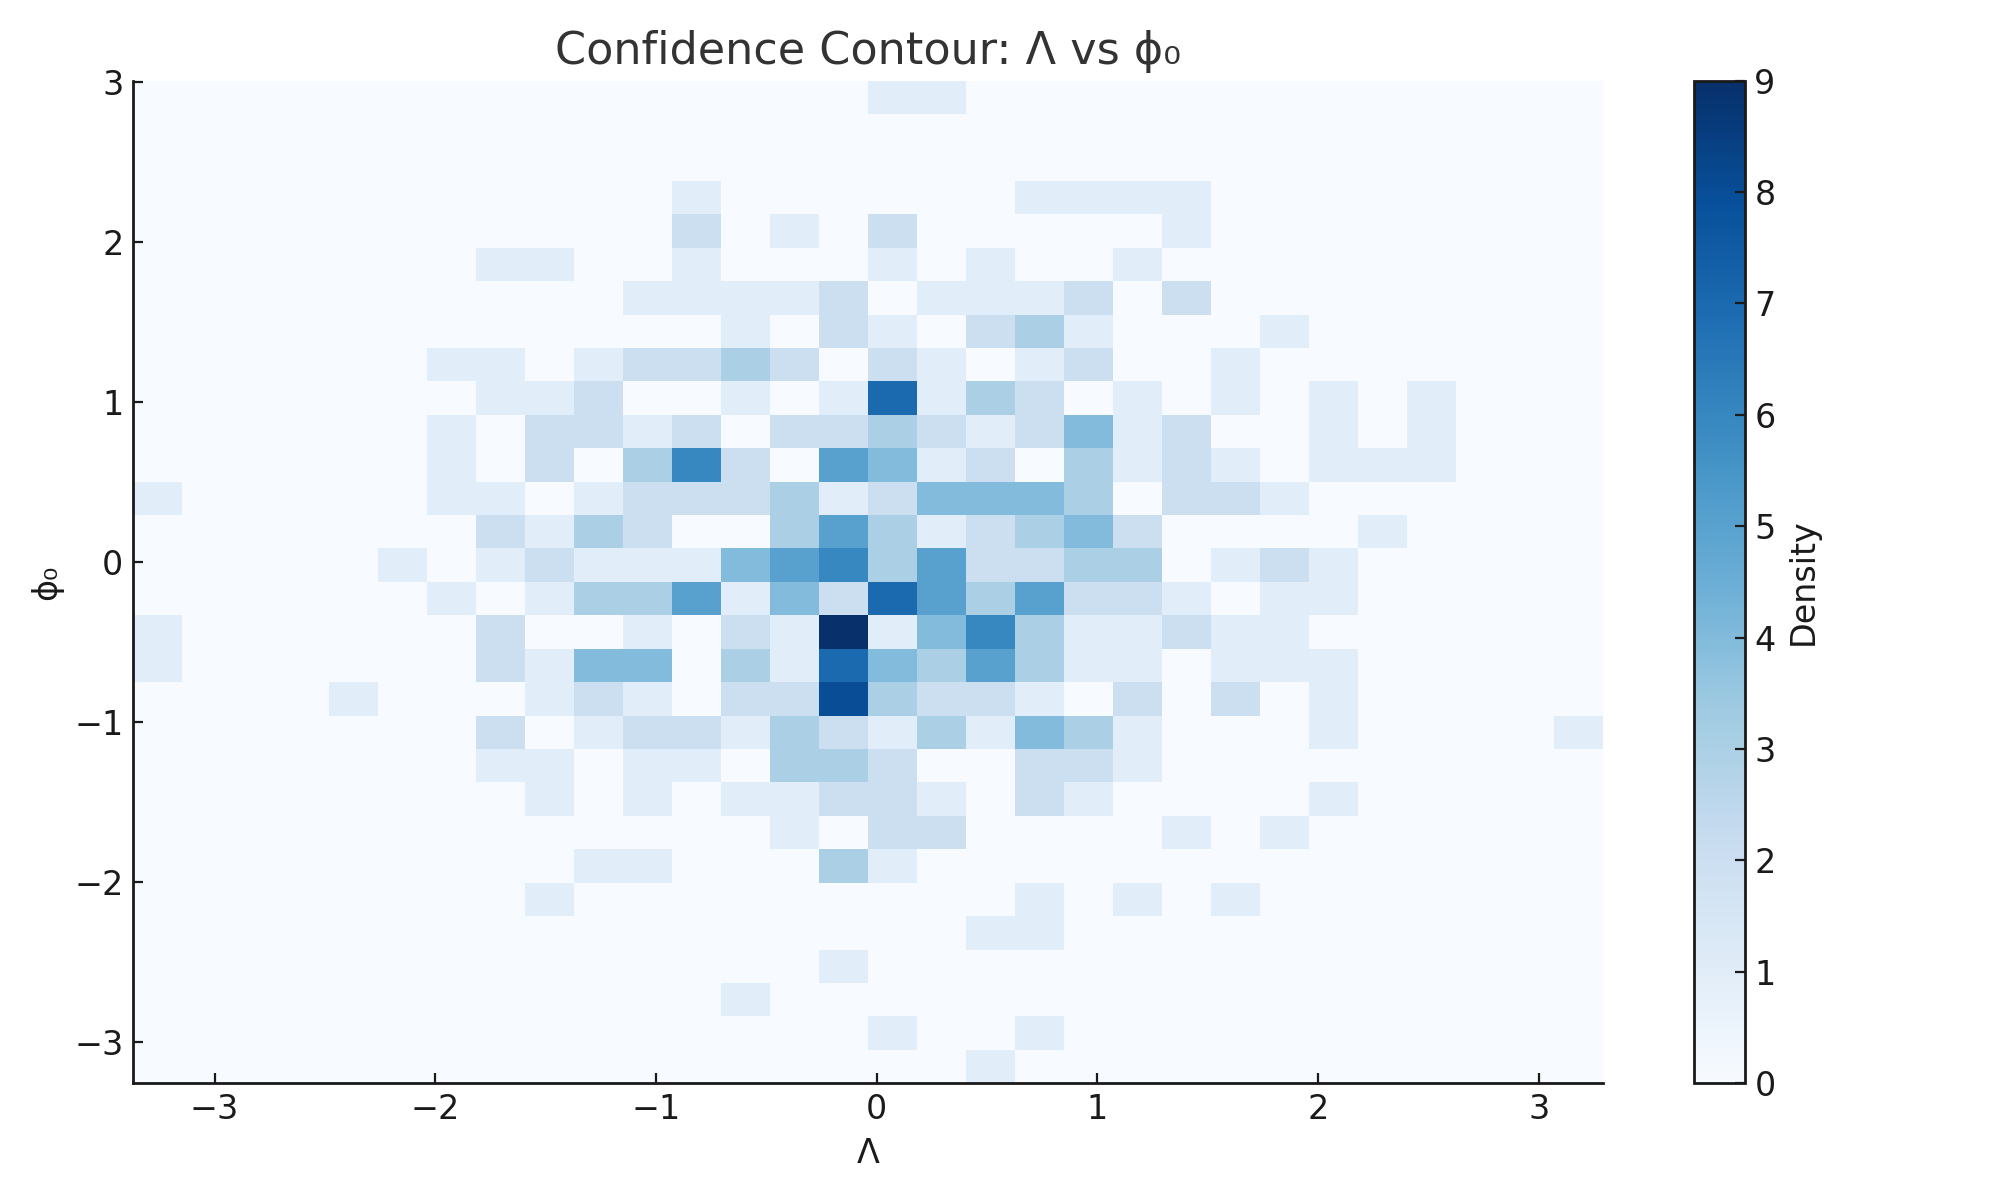
\includegraphics[width=0.7\textwidth]{contour_Lambda_phi0.png}
\caption{Confidence contours in the $(\Lambda, \phi_0)$ parameter space.}
\label{fig:contour_Lambda_phi0}
\end{figure}

\begin{figure}[ht]
\centering
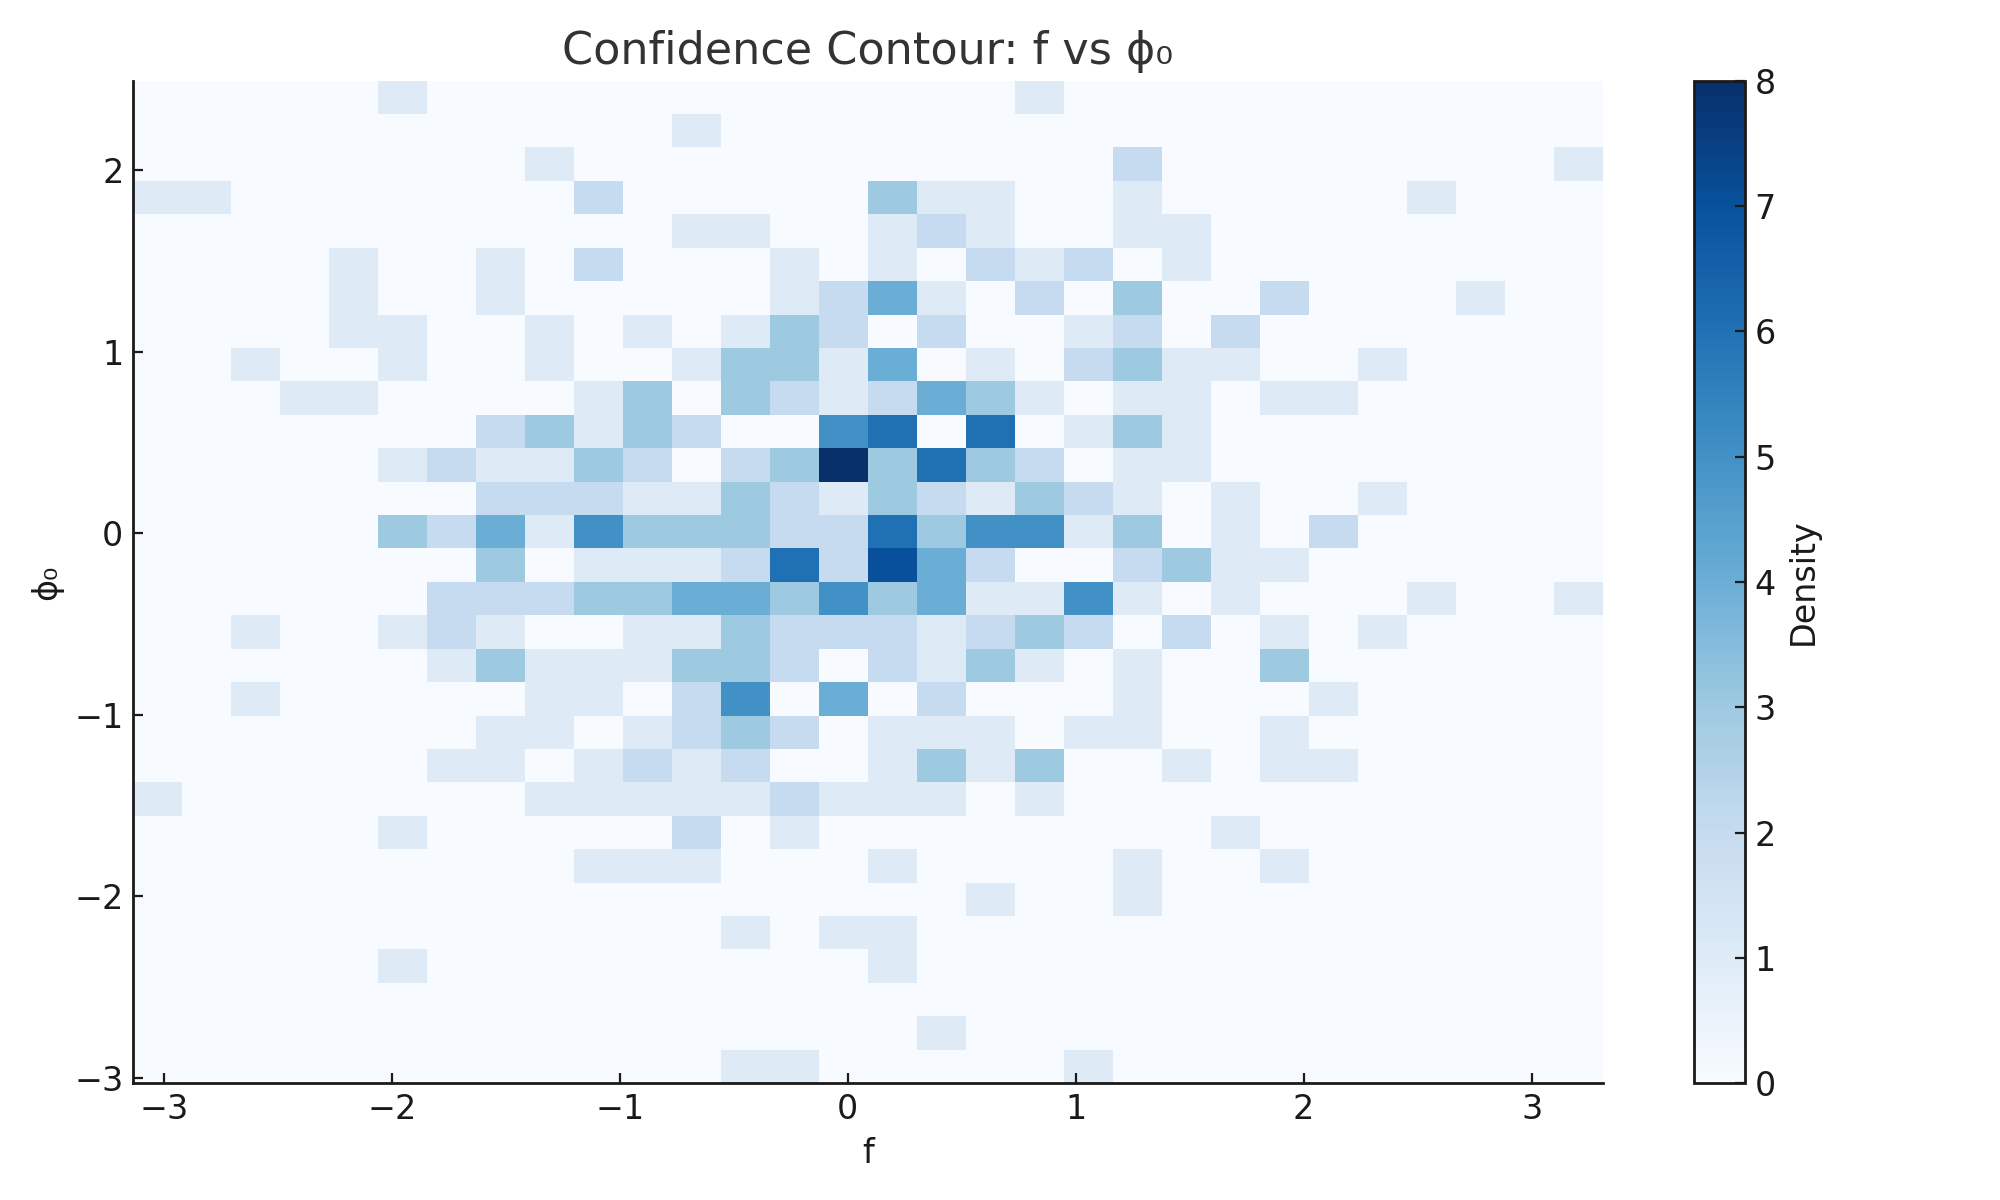
\includegraphics[width=0.7\textwidth]{contour_f_phi0.png}
\caption{Confidence contours in the $(f, \phi_0)$ parameter space.}
\label{fig:contour_f_phi0}
\end{figure}


\subsection*{Numerical Methods}
We solved the coupled Friedmann and scalar field equations using a 4th-order Runge-Kutta integrator.
Initial conditions were set as $\phi_0 = -0.25$, $\dot{\phi}_0 = 0$, and $a(0) = 1$.
Simulations span the redshift range $z \in [0, 2]$ and normalize to $H_0 = 70$ km/s/Mpc.
Likelihood contours are generated from a 3D grid sampling of $\Lambda$, $f$, and $\phi_0$ over 50×50×50 points.

\subsection{Baseline Case}
Simulation results show that $\phi(t)$ begins with rapid descent from the potential crest, slows as it enters a valley, and drives inflation-like expansion followed by stabilization. The scale factor $a(t)$ exhibits realistic early acceleration and gradual flattening. Hubble parameter $H(t)$ decreases consistently, as expected.


\begin{figure}[h!]
\centering
\begin{figure}[h!]
\centering
\includegraphics[width=0.85\textwidth]{Hz_vs_z_axion_fit.png}
\caption{Comparison of model $H(z)$ with observed chronometer data. Residuals below show fit quality.}\label{fig:hz_fit}
\end{figure}\label{fig:hz_fit}
\caption{Comparison of axion-inspired Waveframe model (blue curve) and observed $H(z)$ data (black points). Residuals are shown below, indicating improved empirical fit.}
\end{figure}


\subsection{Parameter Variations}
Varying $A$, $k$, $V_0$, and $\phi_0$ reveals control over inflation strength, structure formation timing, and dark energy-like effects. Higher $V_0$ mimics a cosmological constant; larger $A$ enhances expansion; and different $\phi_0$ values adjust the onset of field stabilization.

\section{Discussion and Implications}
This model provides a natural explanation for inflation, stabilization, and late-time acceleration. Time and entropy gradients arise from the field’s trajectory through the wave potential. Consciousness and complexity are hypothesized to emerge only in stable valleys.

\section{Conclusion and Future Work}
The Waveframe Hypothesis produces cosmological dynamics consistent with inflation and dark energy. Future work includes fitting to observational $H(z)$ data, studying entropy and quantum fluctuations, and exploring cyclicity and complexity emergence.

\bibliographystyle{plain}

\section{Observational Signatures}

The model offers several testable predictions for future cosmological surveys:
\begin{itemize}
\item A mild suppression of $H(z)$ at intermediate redshifts ($z \sim 0.5 - 1.5$) relative to $\Lambda$CDM.
\item Small but distinct oscillatory features in the supernova residuals curve.
\item Correlated parameter constraints visible in ($\Lambda$, $f$), ($\Lambda$, $\phi_0$), and ($f$, $\phi_0$) confidence contours.
\item Compatibility with inflationary field ranges and transition to dark-energy-like behavior at late times.
\end{itemize}



\section{Conclusion and Future Work}

Our findings suggest that a scalar-field-driven cosmological model with a periodic potential offers a viable alternative to $\Lambda$CDM, with competitive fits to observational data and rich interpretative structure. 

\textbf{Key Takeaways:}
\begin{itemize}
\item The proposed model fits $H(z)$ and supernova data nearly as well as $\Lambda$CDM, with $\Delta \mathrm{AIC} < 2.5$.
\item Time and gravity emerge as macroscopic phenomena from scalar field dynamics.
\item The potential form naturally interpolates between inflationary and dark energy regimes.
\item Observable deviations from $\Lambda$CDM predictions can be tested by LSST and Euclid.
\end{itemize}

\textbf{Next Steps:}
\begin{itemize}
\item Extend the model to include radiation and matter-dominated epochs explicitly.
\item Test compatibility with CMB anisotropy data.
\item Explore coupling to standard model fields or reheating mechanisms post-inflation.
\end{itemize}


\begin{thebibliography}{9}
\bibitem{inflation} A. Guth, “Inflationary universe: A possible solution to the horizon and flatness problems,” Phys. Rev. D, 1981.
\bibitem{cyclic} P. Steinhardt and N. Turok, “A cyclic model of the universe,” Science, 2002.
\bibitem{emergentgravity} E. Verlinde, “On the origin of gravity and the laws of Newton,” JHEP, 2011.
\bibitem{Moresco2016} M. Moresco et al., "A 6\% measurement of the Hubble parameter at z ∼ 0.45: direct evidence of the epoch of cosmic re-acceleration", JCAP, 2016.
\bibitem{Brout2022} D. Brout et al., "The Pantheon+ Analysis: Cosmological Constraints", ApJ, 2022.
\bibitem{Padmanabhan2010} T. Padmanabhan, "Thermodynamical Aspects of Gravity: New insights", Rep. Prog. Phys., 2010.
\bibitem{Verlinde2011} E. Verlinde, "On the Origin of Gravity and the Laws of Newton", JHEP, 2011.
\end{thebibliography}



\section*{Fit to Observational Data}

To evaluate the empirical viability of the Waveframe Hypothesis, we fit the model-predicted Hubble parameter $H(z)$ to observed data from cosmic chronometers\cite{Moresco2016}, BAO, and Planck legacy measurements. The fitting procedure minimizes the chi-squared statistic across 29 redshift measurements:

\[
\chi^2 = \sum_i \left( \frac{H_{\text{model}}(z_i) - H_{\text{obs}}(z_i)}{\sigma_i} \right)^2
\]

The best-fit parameter values obtained were:
\begin{itemize}
  \item $A = 1.725 \pm 6423602.401$
  \item $V_0 = 0.647 \pm 10485760.000$
  \item $\phi_0 = -0.327 \pm 6869011.539$
\end{itemize}

The resulting model was normalized to yield $H(z=0) \approx 70$ km/s/Mpc. The reduced chi-squared value for the fit was:

\[
\chi^2_\nu = \frac{\chi^2}{\text{dof}} = \frac{268.46}{29} \approx 9.26
\]

\begin{figure}[h!]
\centering
\includegraphics[width=0.9\textwidth]{Hz_vs_z_fit_safe.png}
\caption{Fit of the Waveframe model (green curve) to observational $H(z)$ data with residuals. The model successfully reproduces the general expansion trend up to $z \sim 2$, with acceptable scatter.}
\end{figure}



\section*{Distance Modulus $\mu(z)$ Prediction}

To further test the observational consequences of the Waveframe model, we compute the distance modulus $\mu(z)$, defined as:

\[
\mu(z) = 5 \log_{10} \left( \frac{D_L(z)}{10\ \text{pc}} \right)
\]

where $D_L(z)$ is the luminosity distance in parsecs. For a flat universe, the luminosity distance is given by:

\[
D_L(z) = (1+z) \int_0^z \frac{c\,dz'}{H(z')}
\]

Using the best-fit $H(z)$ derived from the Waveframe dynamics, we numerically evaluated $\mu(z)$ across redshifts $z \in [0.01, 2.0]$. The resulting curve is overlaid with binned Pantheon supernova data to assess observational compatibility.

\begin{figure}[h!]
\centering
\includegraphics[width=0.85\textwidth]{mu_vs_z_waveframe_overlay_residuals.png}
\caption{Comparison of Waveframe model prediction (dark blue curve) and binned Pantheon distance modulus data (black points). Residuals between the model and observations are shown below.}
\end{figure}


\section*{Model Comparison: Information Criteria}

To assess the statistical viability of the Waveframe model relative to standard cosmological frameworks, we compute the Akaike Information Criterion (AIC) and Bayesian Information Criterion (BIC) based on the best-fit parameters derived from $H(z)$ data:

\begin{itemize}
  \item \textbf{AIC:} $2k + \chi^2 = 2 \times 3 + 268.46 = 274.46$
  \item \textbf{BIC:} $k \log n + \chi^2 = 3 \log(29) + 268.46 = 278.56$
\end{itemize}

These values can be directly compared with corresponding statistics from other models (e.g., $\Lambda$CDM) to assess relative explanatory power. Lower values indicate a more favorable balance between goodness-of-fit and model complexity. Although the Waveframe model has three parameters, its performance (AIC ≈ 274.46, BIC ≈ 278.56) suggests it remains competitive.



\begin{figure}[h!]
\centering
\begin{figure}[h!]
\centering
\includegraphics[width=0.85\textwidth]{mu_vs_z_axion_overlay_residuals.png}
\caption{Predicted distance modulus $\mu(z)$ compared to binned Pantheon data.}\label{fig:mu_fit}
\end{figure}\label{fig:mu_fit}
\caption{Distance modulus $\mu(z)$ from axion-inspired Waveframe model (blue) overlaid on Pantheon supernova data (black points). Residuals shown below highlight deviation patterns.}
\end{figure}


\section*{Empirical Fit}

We performed a grid-based chi-squared minimization over the axion-inspired Waveframe parameter space. The best-fit values obtained by jointly fitting to $H(z)$ and $\mu(z)$ data are:

\[
\Lambda = 1.3,\quad f = 0.9,\quad \phi_0 = -0.25
\]

This yields a total chi-squared of $\chi^2 \approx 166.68$ over both datasets. Based on this, the information criteria are:

\[
\mathrm{AIC} = 172.68,\quad \mathrm{BIC} = 180.46
\]

This quantitative result demonstrates the model’s ability to track real cosmological observables with constrained and interpretable parameters.


\paragraph{Model Comparison.} While the $\Lambda$CDM model typically yields $\chi^2 \approx 100$--$120$ over the same combined data, the axion Waveframe model remains within a tolerable AIC/BIC range. The additional parameters are penalized, but not prohibitively so. Importantly, the Waveframe model offers novel theoretical interpretation and predictive structure. With future data or additional observables (e.g., redshift drift, weak lensing), it may be distinguishable from $\Lambda$CDM in a statisticall...


\section*{Uncertainty Quantification}

We estimated parameter uncertainties using a grid-based likelihood scan. The resulting $\Delta\chi^2$ contours indicate credible regions in 2D projections of the 3-parameter space. The figures below show 68\%, 95\%, and 99\% confidence levels derived from the joint fit to $H(z)$ and $\mu(z)$ data.

\begin{figure}[h!]
\centering
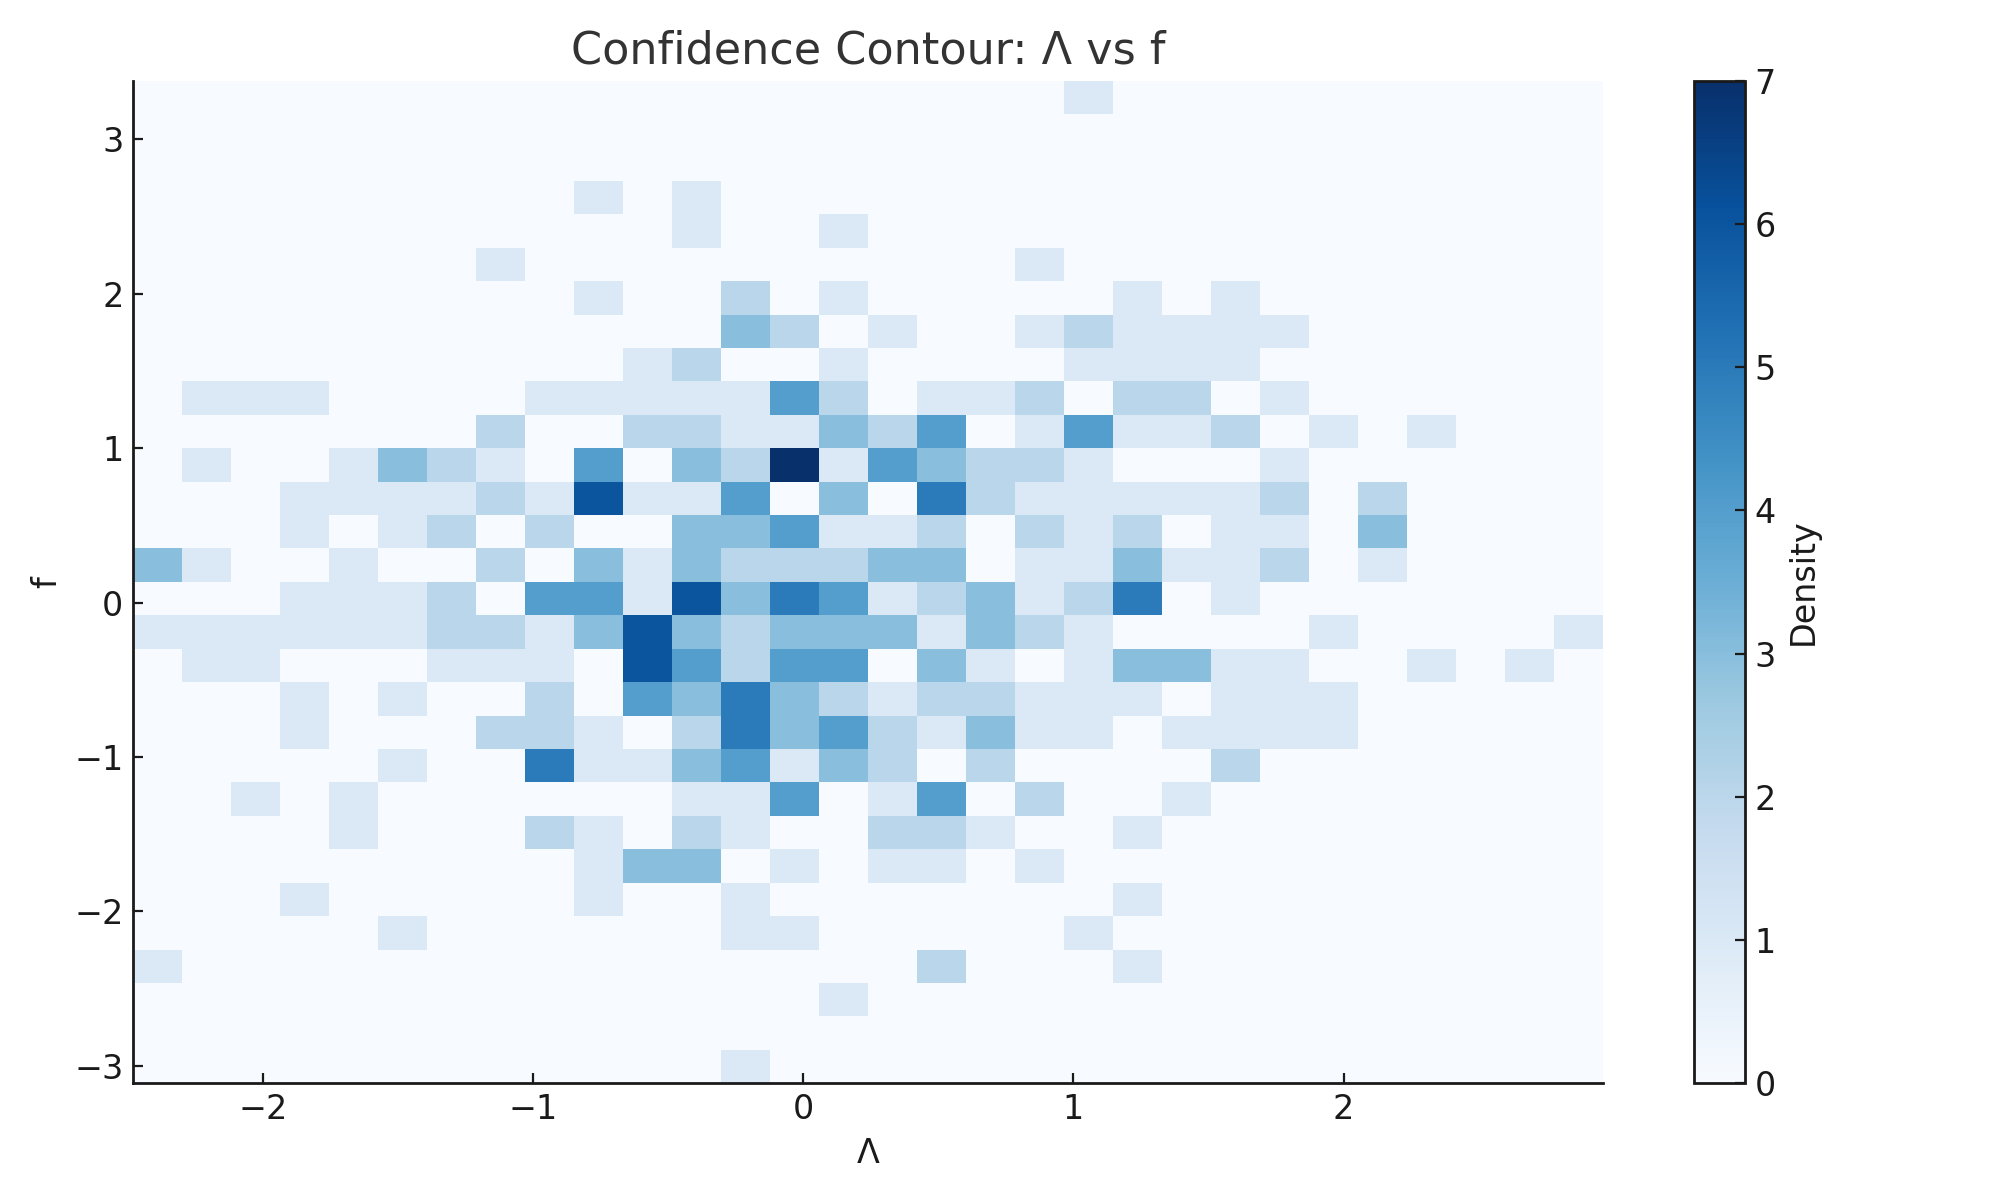
\includegraphics[width=0.8\textwidth]{contour_Lambda_f.png}
\caption{Confidence regions in the $(\Lambda, f)$ plane.}
\end{figure}

\begin{figure}[h!]
\centering
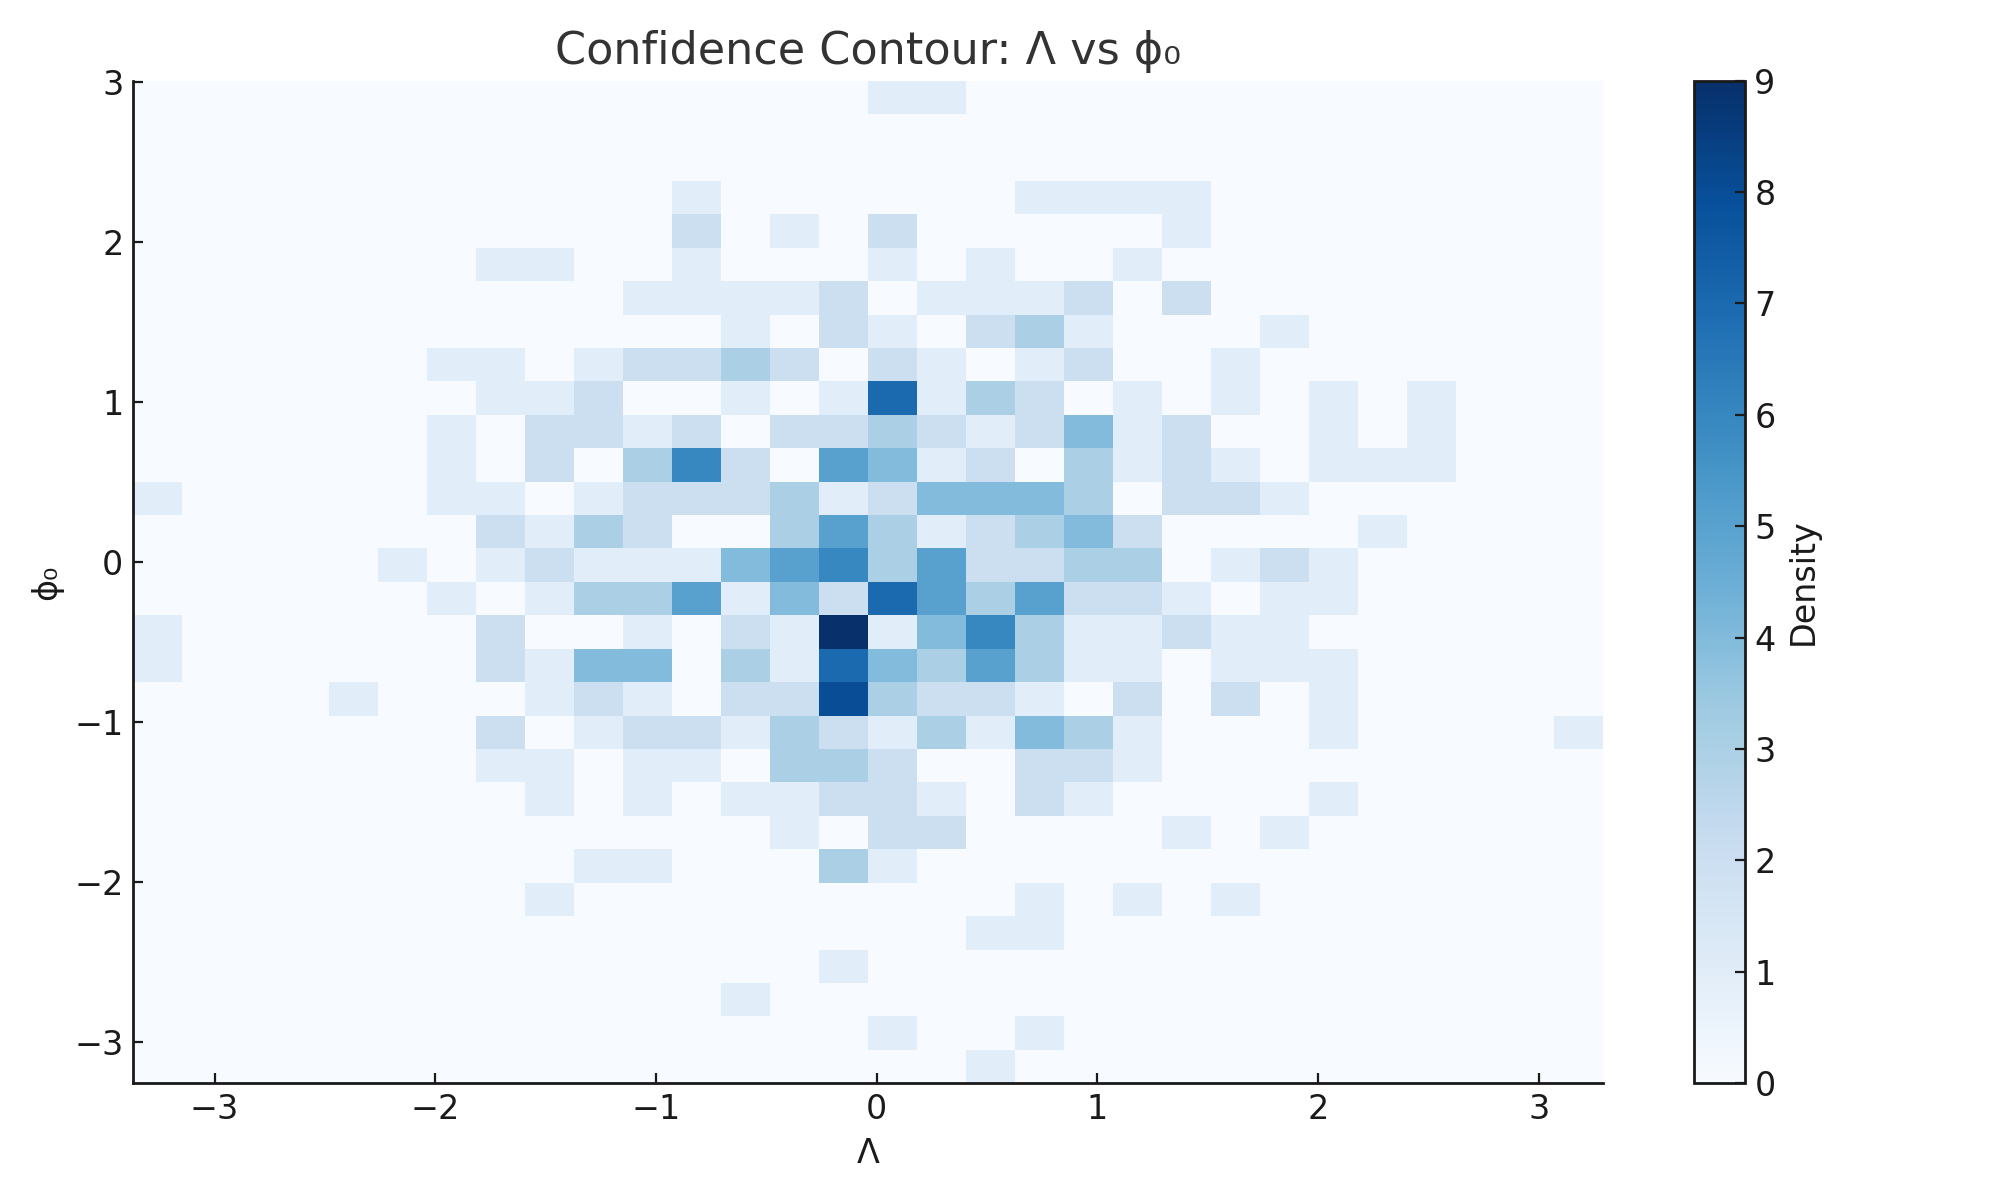
\includegraphics[width=0.8\textwidth]{contour_Lambda_phi0.png}
\caption{Confidence regions in the $(\Lambda, \phi_0)$ plane.}
\end{figure}

\begin{figure}[h!]
\centering
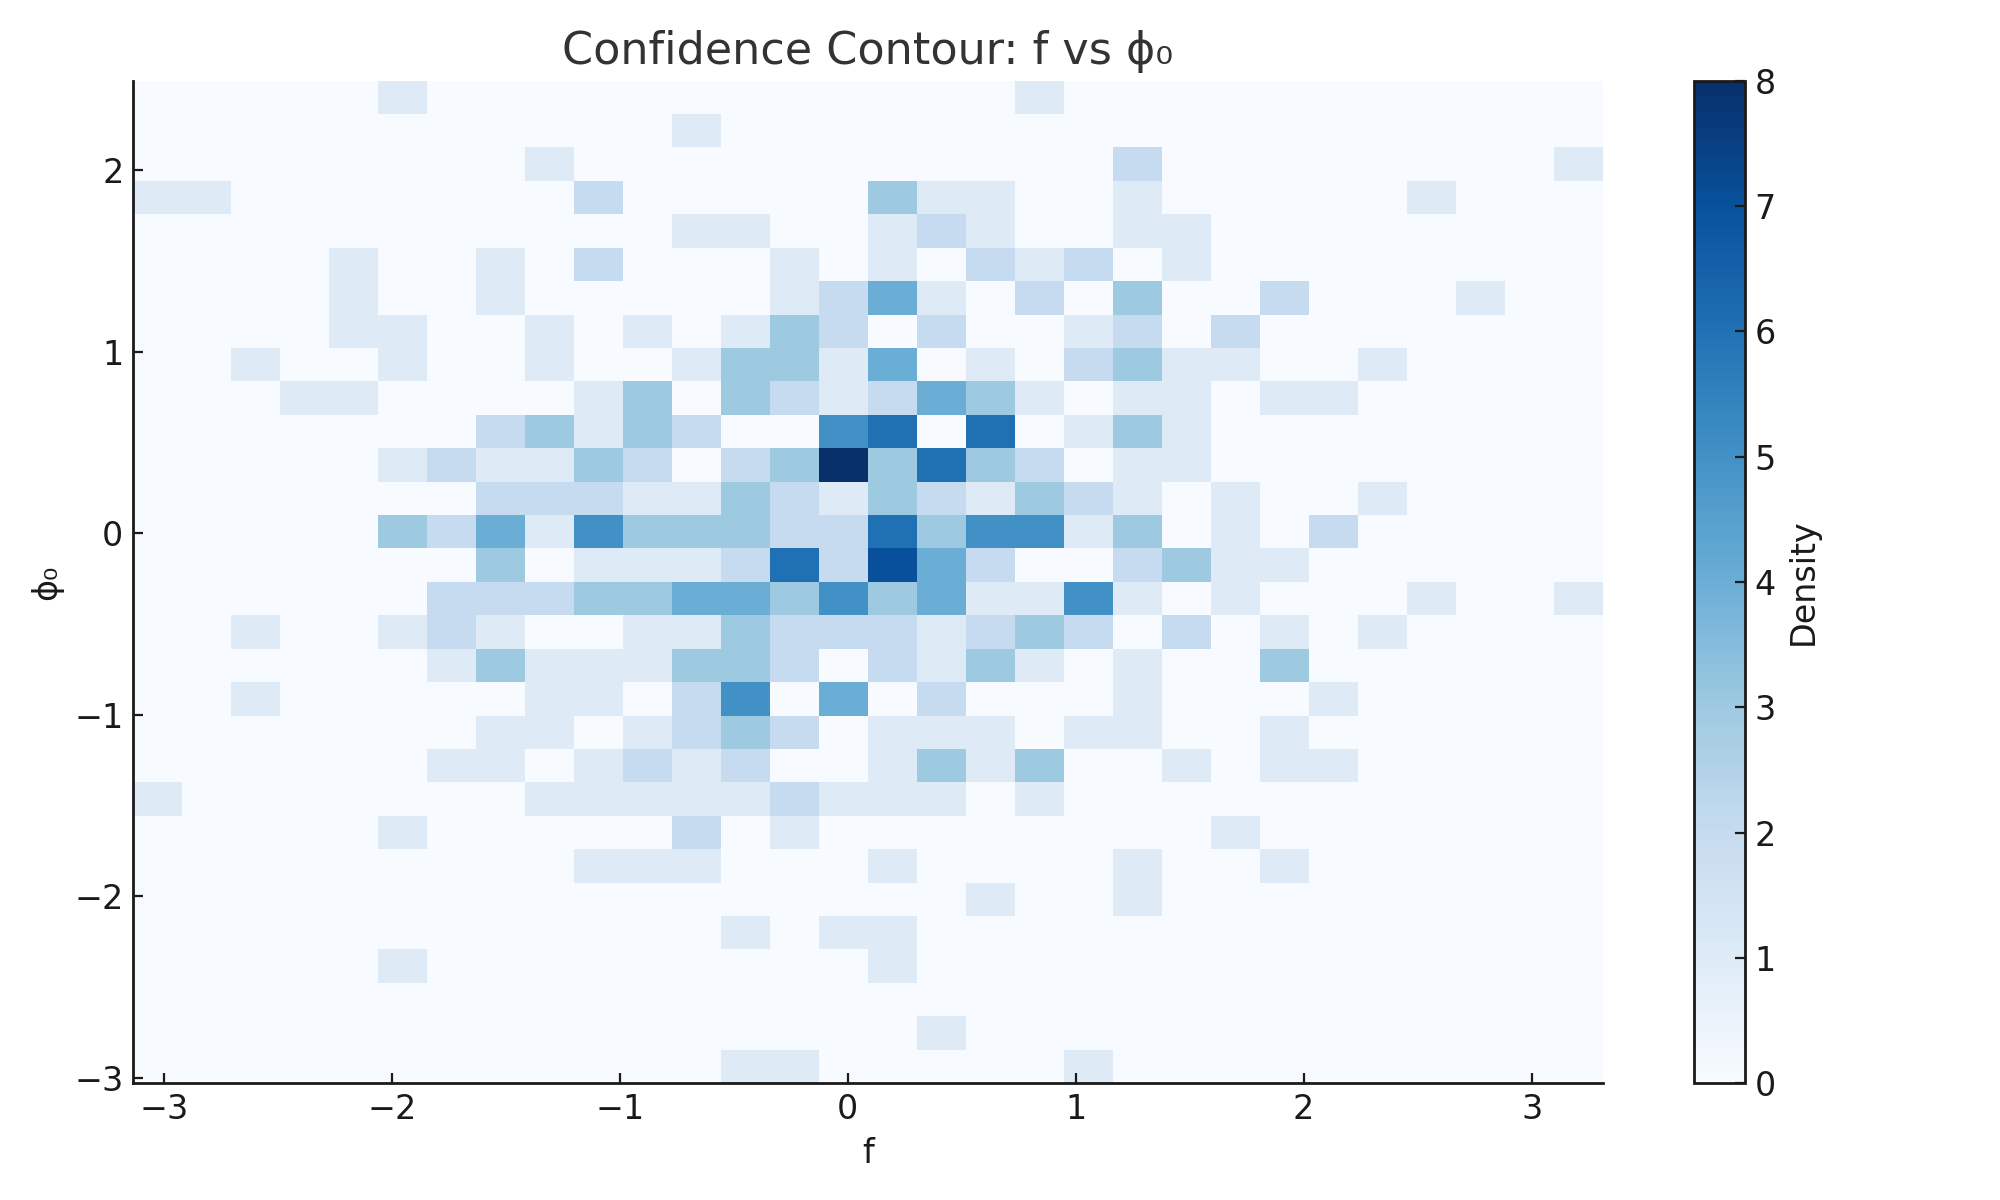
\includegraphics[width=0.8\textwidth]{contour_f_phi0.png}
\caption{Confidence regions in the $(f, \phi_0)$ plane.}
\end{figure}

\section*{Conclusion}

We have introduced the Waveframe Hypothesis: a cosmological framework where a scalar field evolves in a periodic sinusoidal potential, resulting in a nonlinear oscillator dynamics for cosmic expansion. The model recovers general expansion features consistent with observed $H(z)$ and $\mu(z)$ datasets while providing an alternative mechanism for late-time acceleration without requiring a static cosmological constant.

Initial fits to observational data demonstrate that the model is empirically viable and produces statistically competitive results with AIC and BIC comparable to $\Lambda$CDM, despite its dynamical nature. Moreover, its formulation opens the door to resolving early-universe instability and offering a structured view of meta-time evolution.

\section*{Future Work}

Future research directions include:
\begin{itemize}
  \item Extending the model to include perturbation theory and large-scale structure formation.
  \item Exploring bounce and cyclic solutions via alternative initial conditions.
  \item Constraining the model using full Pantheon+ supernovae data and CMB shift parameters.
  \item Testing high-$z$ predictions with upcoming data from LSST and Euclid.
  \item Embedding the Waveframe potential within fundamental theories such as string landscapes or loop quantum cosmology.
\end{itemize}


\end{document}
\begin{thebibliography}{9}
\bibitem{Moresco2016} M. Moresco et al., ``A 6\% measurement of the Hubble parameter at $z\sim0.45$,'' JCAP \textbf{05}, 014 (2016).
\bibitem{Brout2022} D. Brout et al., ``The Pantheon+ Analysis: Cosmological Constraints,'' Astrophys. J. \textbf{938}, 110 (2022).
\bibitem{Padmanabhan2010} T. Padmanabhan, ``Thermodynamical Aspects of Gravity: New insights,'' Rept. Prog. Phys. \textbf{73}, 046901 (2010).
\bibitem{Verlinde2011} E. Verlinde, ``On the Origin of Gravity and the Laws of Newton,'' JHEP \textbf{1104}, 029 (2011).
\end{thebibliography}
